\begin{problem}{Illumination}{\textsl{standard input}}{\textsl{standard output}}{2 seconds}{512 mebibytes}{}

In the room, shaped as the simple polygon with $N$ vertices (i.e. closed
polyline without self-intersections), an light source is put in the 
point $(X_c,Y_c)$. Find out an area of illuminated part of the room.

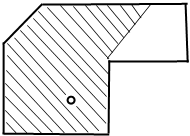
\includegraphics{i.png}


\InputFile

First line of the input file contains one integer $T$ --- number of the
test cases ($1 \le T <200$). First line of each test case contains 
two real numbers $X_c$ and $Y_c$ --- coordinates of the light source.
Next line contains one integer $N$ --- number of vertices of the polyline
($3 \le N \le 5 \cdot 10^4$). Each of the next $N$ lines contain
coordinate of one vertices of the polyline --- two real numbers
$X_i$ and $Y_i$. All coordinates are given with no more than 4 digits
after the decimal point and does not exceed 1000 by absolute value. 
It is guaranteed that light source is strictly inside the room.

\OutputFile

For each test case print one integer --- area of illuminated part of the room
with precision $10^{-2}$ or better.


\Examples
\begin{example}
\exmp{
1
1 2
5
0 0
1 0
1 1
3 3
0 3
}{
5.00
}%
\end{example}
\end{problem}
